\documentclass{llncs}
\usepackage{amssymb}
\usepackage[utf8]{inputenc}
\usepackage{url}
\usepackage{graphicx}
\usepackage{caption}
\usepackage{subcaption}
\usepackage{epstopdf}
\usepackage{subfig}
\usepackage{float}
\usepackage{amsmath}
\usepackage{wrapfig}
\usepackage{fancyhdr} %Usado para configurar encabezado y pie de página


\pagestyle{empty}
\pagestyle{fancy}
%\rfoot{\thepage}

\begin{document}

\title{Pumas@Home 2017 Team Description Paper}
\author{
	Jesus Savage 
	\and Marco Negrete 
	\and Hector Arce 
	\and Reynaldo Martell 
	\and Hugo Estrada 
	\and Julio Cruz 
	\and Manuel Pano 
	\and Jaime Marquez 
	\and Edgar Silva
	\and Edgar Vazquez
	\and Jose Luis Cruz
}
\institute{National Autonomous University of Mexico, México DF 04510, MEX, \\
\texttt{http://biorobotics.fi-p.unam.mx}}
\maketitle


%%%%%%%%%%%%%
%%%  ABSTRACT  %%%
%%%%%%%%%%%%%
\begin{abstract}
This robot is based on the ViRBot architecture, implemented by several modules that perform different tasks, using the ROS platform, together with a cross-platform system called Blackboard developed by us. This year, several improvements in hardware and software of Robot Justina has been made. Currently, our research is mainly focused on task planning using different approaches and the development of a framework to test and debug the execution of the plans.
\end{abstract}

%%%%%%%%%%%%%%%
%%% INTRODUCTION %%%
%%%%%%%%%%%%%%%

\section{Introduction}

The service robots are hardware and software systems that can assist humans to perform daily tasks in complex environments. To achieve this, a service robot has to be capable of understanding commands from humans, avoiding static and dynamic obstacles while navigating in known and unknown environments, recognizing and manipulating objects and performing several other tasks that a person might request. This paper describes the autonomous service robot Justina and the research of the Team Pumas, which has been participating in RoboCup@Home league since 2007. It is organized as follows:

In section \ref{sec:background} the ViRBot architecture is described as the platform for the robot software system. Section \ref{sec:Justina} enumerates the hardware and software components of robot Justina, and the functionality of each of them is described. Section \ref{sec:CurrentResearch} is an abstract of the latest research developed in our laboratory in order to improve the robot's performance and finally, in section \ref{sec:conclusions}, conclusions and future work are given.

%%%%%%%%%%%%%%%%%%
%%% BACKGROUND %%%
%%%%%%%%%%%%%%%%%%

\section{Background: Platform and Architecture}\label{sec:background}

This robot is based on the ViRBot architecture for autonomous mobile robot operation \cite{virbot}, which provides a platform for the design and development of software for general purpose service robots. 

The ViRBot architecture defines a human-robot interaction interface made of three main layers (see figure \ref{fig:virbot}):

\begin{itemize}
	\item \textbf{Input layer:} Includes all algorithms related to the acquisition of data from the environment. 
	\item \textbf{Planning and Knowledge:} This layer performs most of the AI algorithms.
	\item \textbf{Execution:} Includes low-level control and supervision. 
\end{itemize}

\begin{figure}[h]
	\centering
	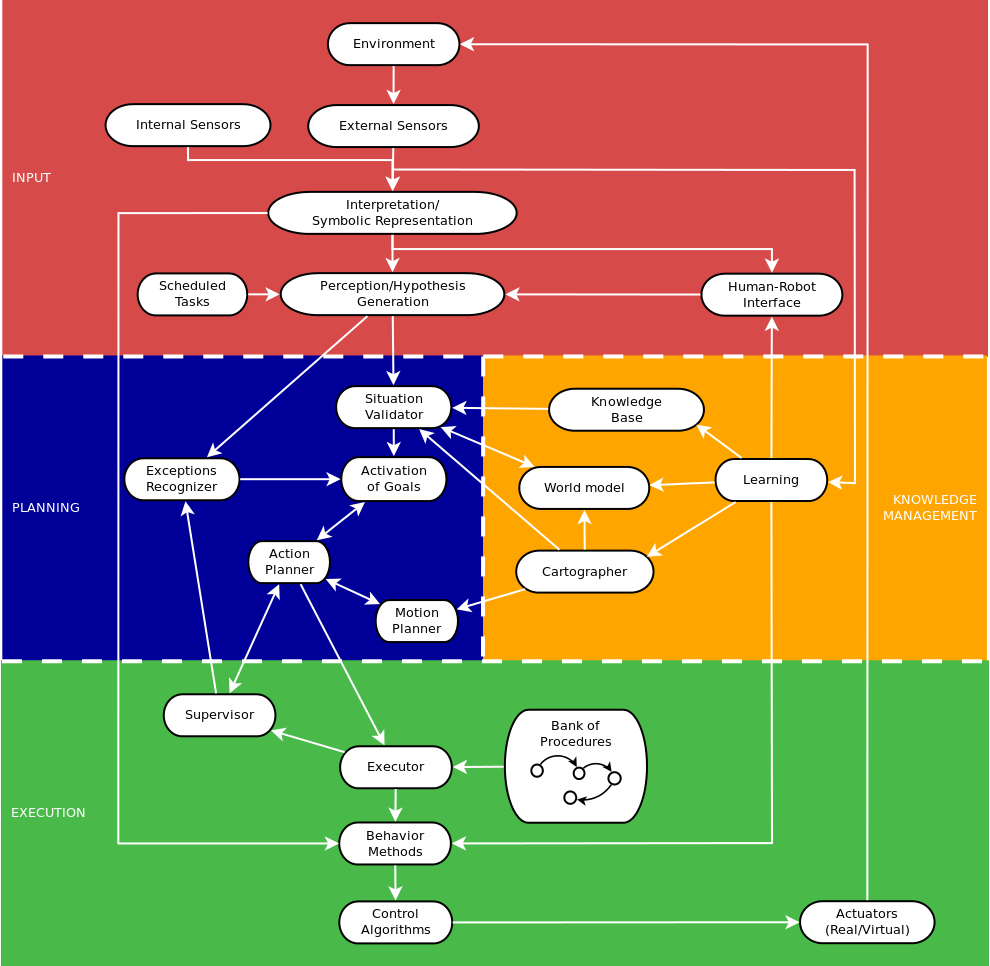
\includegraphics[width=0.8\textwidth]{Figures/ViRBot.png}
	\caption{Block diagram of the ViRBot architecture.}
	\label{fig:virbot}
\end{figure}

The ViRBot architecture is implemented in our robots through several modules that perform well defined tasks, with a high level of interaction between them. The principal framework used for interaction is ROS, where a Module is represented by one or several ROS' nodes.

Also, we make extensive use of our self-made Framework for modules interaction called Blackboard (BB). In BB, the information exchange is made through a central module which supports shared variables, publisher/subscriber pattern, and message passing. BB was developed mainly in C\# and the .NET framework, with APIs to build BB modules for C\#, C++ and Python 2.7. It runs on Windows and Unix-based systems (with the help of Mono, an open source implementation of Microsoft's .NET framework). Currently, we had tested BB modules running on Windows, Ubuntu, Mac-OS, Android and Raspbian

BB's commands and shared variables have a certain equivalence to ROS' services and topics respectively. Integration between ROS nodes and BB modules has been accomplished through the implementation of the Blackboard Bridge module, which is a ROS node written in C++ with the BB Module API.

%%%%%%%%%%%%%%
%%%%	JUSTINA %%%%
%%%%%%%%%%%%%%

\begin{figure}[h]
	\centering
	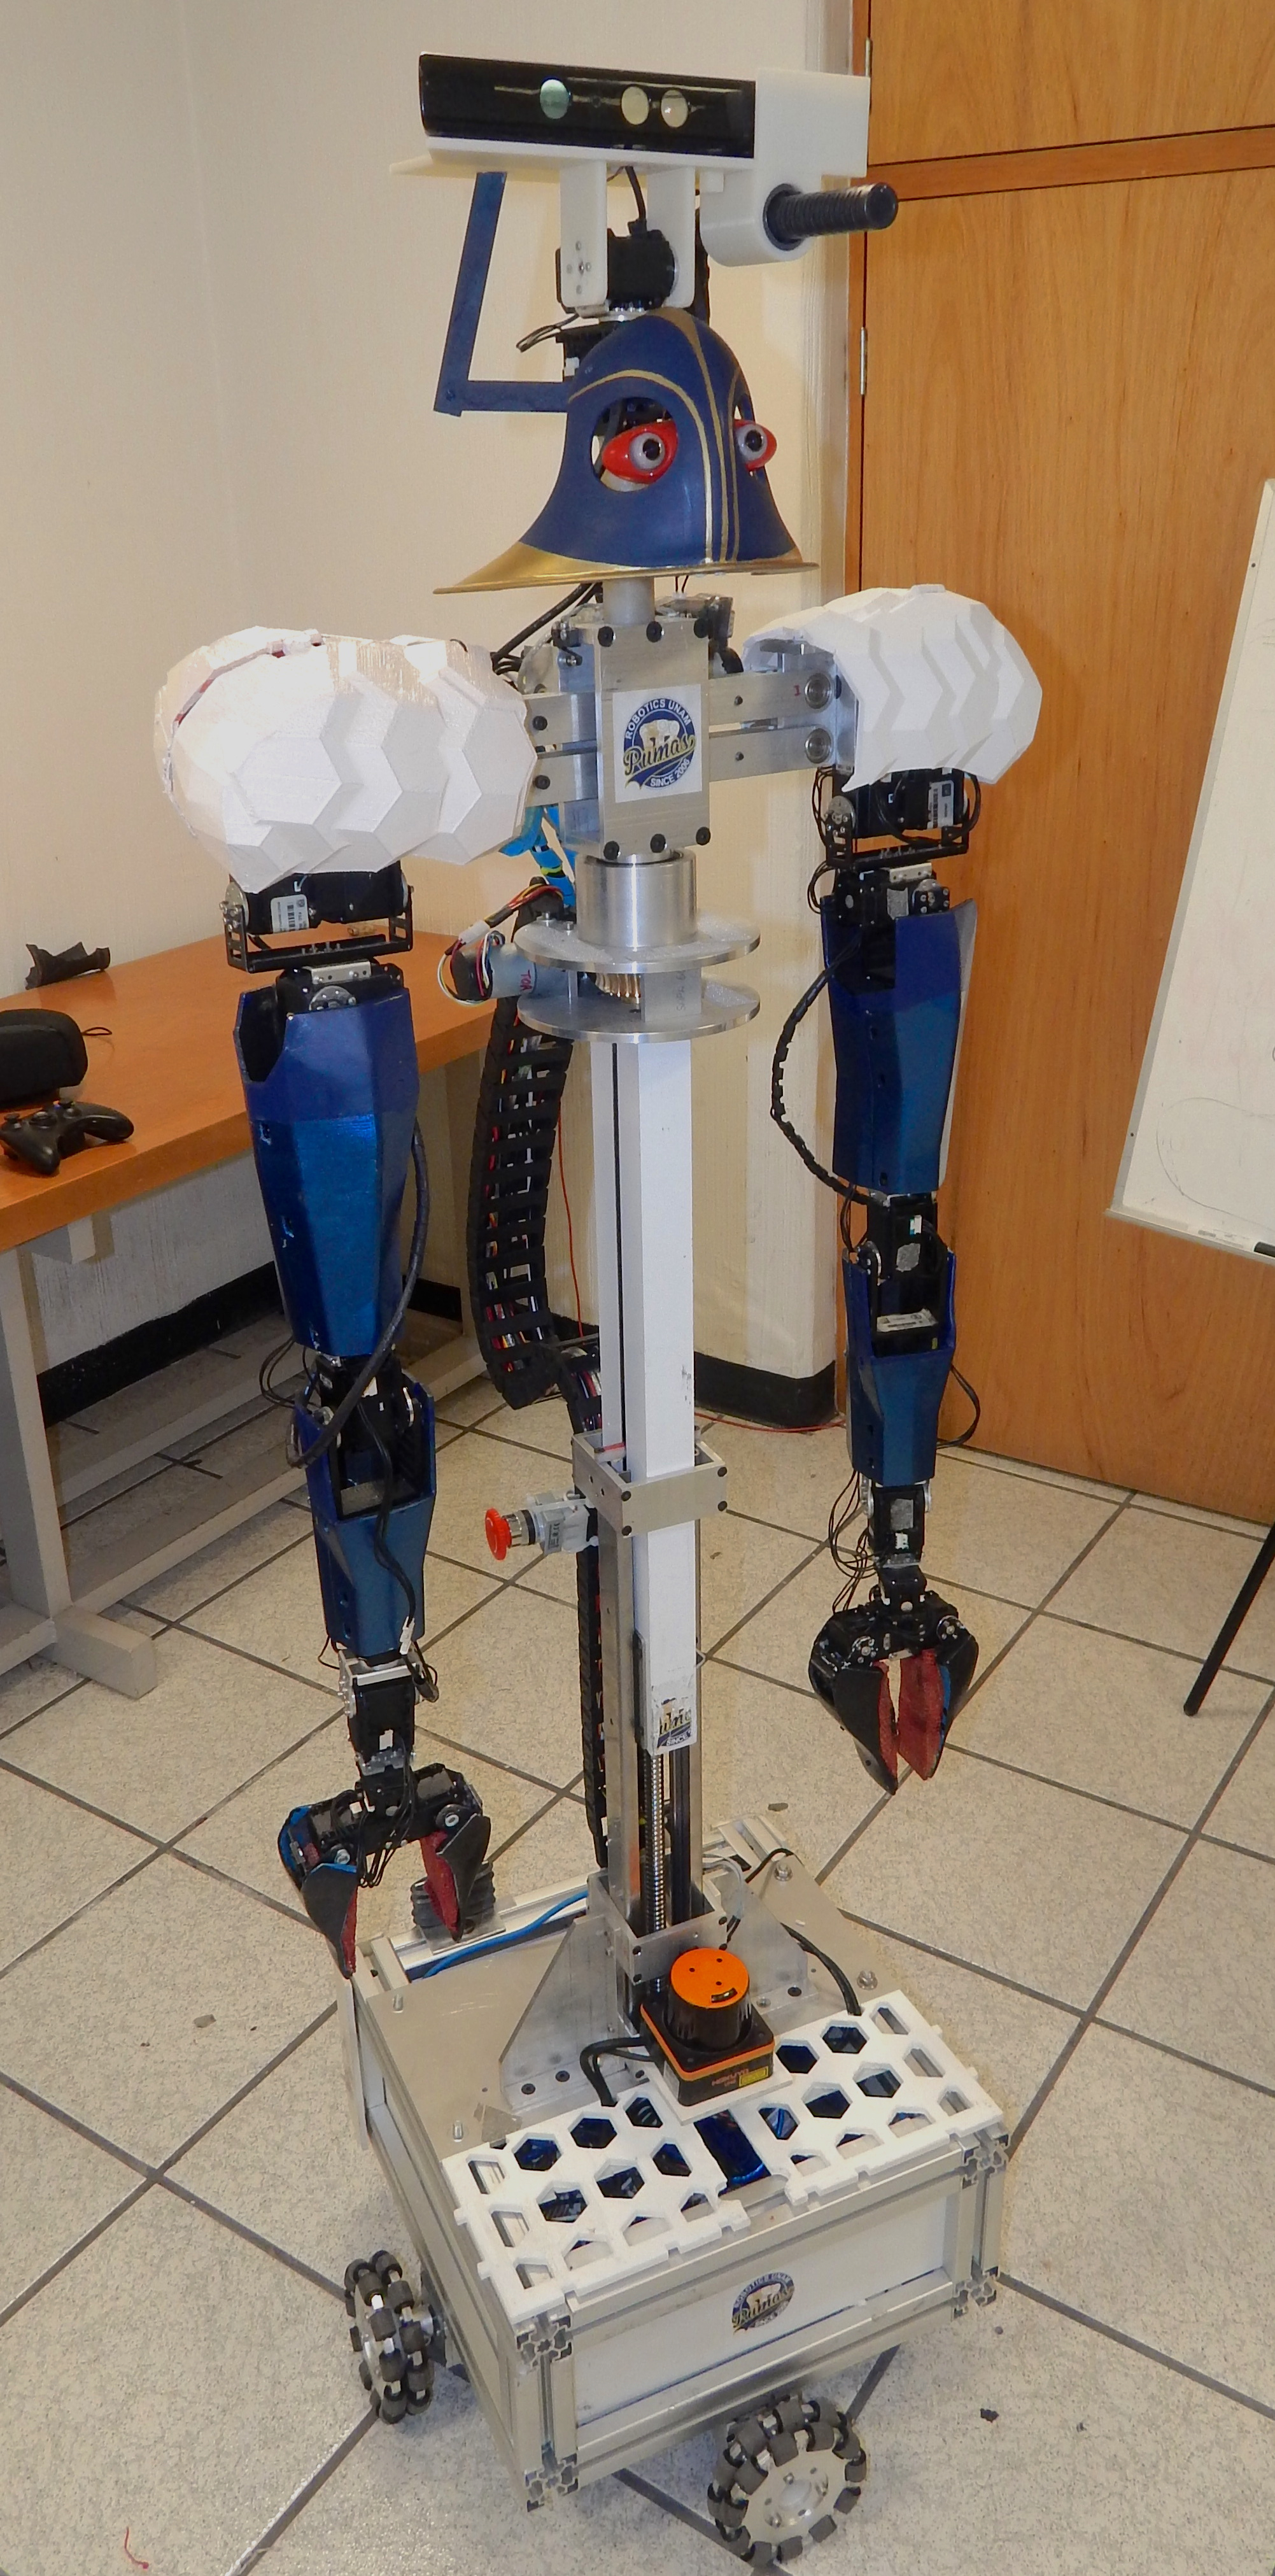
\includegraphics[width=0.45\textwidth]{Figures/justina2017.jpg}
	\caption{Robot Justina}
	\label{fig:justina}
\end{figure}

\section{Robot Justina}\label{sec:Justina}

%%% ACTUATORS
\subsection{Actuators}

\begin{itemize}
	\item \textbf{Mobile base:} Omnidirectional through differential pair configuration and omnidirectional wheels (self design). 
	\item \textbf{Manipulators:} 2 x 7-DOF anthropomorphic arms with 10 Dynamixel servomotors each.
	\item \textbf{Head:} 2-DOF (Pan and tilt) built with Dynamixel servomotors.
	\item \textbf{Torso:} 3-DOF (Elevation, pan, and shoulders tilt) through a worm screw and a configuration of gears. 
	\item \textbf{Remote:} Xbox wireless remote controller.
\end{itemize}

%%% SENSORS
\subsection{Sensors}

\begin{itemize}
	\item \textbf{RGB-D Camera:} Microsoft's Kinect sensor 
	\item \textbf{RGB Camera:} Logitech Pro C920 Full HD.
	\item \textbf{Microphone:} Rode NTG2 directional microphone.
	\item \textbf{Laser:} Hokuyo rangefinder URG-04LX-UG0.
\end{itemize}

%%% SOFTWARE
\subsection{Software}

Robot Justina uses two computers: one running Ubuntu 14.04 and one running Windows 7. Modules are programmed in C\#, C++, Python or CLIPS \cite{clips}. Modules currently running on Justina are:

\begin{description}
	\item[Action Planner] Details are given in subsection \ref{subsec:ActionPln}. 
	\item[Simple Task Planner] Bank of procedures that involves simple and repetitive tasks easily achieved by state machines, e.g. grasping an object, searching for a face, aligning with an edge, etc.
	\item[Motion Planner] Path planning for the non-linear control of the mobile base. Also, some obstacle avoidance behaviours are implemented using point cloud data of the scene. 
	\item[Object Finder] Details are given in subsection \ref{subsec:objDet}
	\item[Person Finder] Multiple face detection using a Haar cascades like algorithm. Face recognition and the online training is performed using 2D and 3D data from the Kinect sensor. 
	\item[Speech Recognition] Throws hypothesis (text strings) of recognized voice with a confidence ranking using Microsoft SAPI 5.3 \cite{SAPI} (commercial software).
	\item[Speech Generator] Voice synthesizer using Microsoft SAPI 5.3 \cite{SAPI} with the Loquendo Susan voice (commercial software).
	\item[Cartographer] Map building and localization based on GMapping node.
	\item[Leg Finder] Legs of pedestrians in a scene are detected and localized using the laser readings.  
\end{description}

%%%%%%%%%%%%%%%%%%%
%%% CURRENT RESEARCH  %%%
%%%%%%%%%%%%%%%%%%%

\section{Current research}\label{sec:CurrentResearch}

%%% CHORO DEL SR. HUGO
\subsection{Surface reconstruction on virtual environments}\label{subsec:SurfRecon}
This research has as main purpose to build a 3D representation of an environment, in which a service robot can interact, using the data obtained by a wide variety of sensors.

Particularly, the data that we use in our experiments are point clouds sets. The capture of this data is performed by the Kinect sensor of robot Justina. To align several captures of point clouds of a scene, an implementation of the ICP (Iterative Closest Point) algorithm is used. Also, a sampling step is implemented using Vector Quantization \cite{linde1980algorithm}. The virtual environment built can be visualized using the simulator described in subsection \ref{subsec:Simulator} . 

The system was successfully tested experimentally by reconstructing our laboratory. Figure 
\ref{fig:SurfRecon} shows an image of multiple point clouds sets captured by the robot and the virtual environment created after the method described above.

\begin{figure}
	\centering
	\begin{subfigure}{0.49\textwidth}
		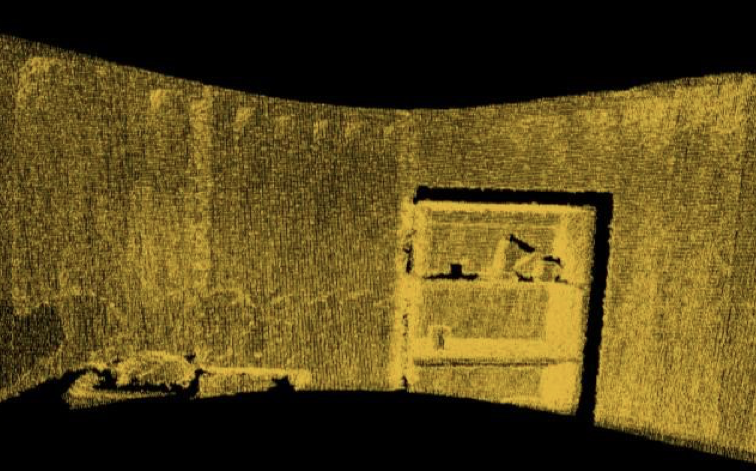
\includegraphics[width=\textwidth]{Figures/envReco1.png} 
		\caption{ Several point clouds captures of a scene.}
		\label{fig:SurfRecon1}
	\end{subfigure}
	\begin{subfigure}{0.49\textwidth}
		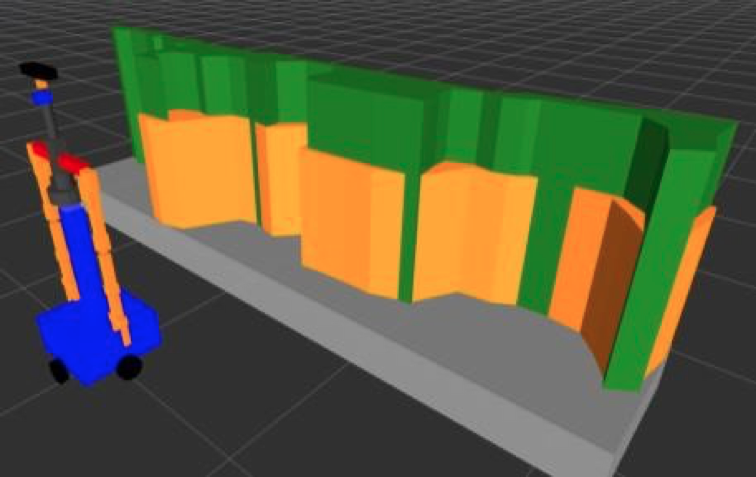
\includegraphics[width=\textwidth]{Figures/envReco2.png}
		\caption{Virtual environment build after processing the sets.}
		\label{fig:SurfRecon2}
	\end{subfigure}
	\caption{Example of the test performed in a real scene.}
	\label{fig:SurfRecon}
\end{figure}

%%% CHORO DEL SR. REYNALDO

\subsection{Service Mobile Robot Simulator}\label{subsec:Simulator}

We developed a new software for simulation and graphical representation of algorithms and behaviours used   in autonomous service robot navigation in dynamic environments. This simulator allow us and new robotics students to test and improve behaviours for the navigation module of robot Justina.

This new simulator has implemented several features such as laser range finder simulations, obstacle representation and rendering using point clouds sets, collision detection, kinematics models for certain mobile base configurations, etc, polygons growing. Also, a graphical user interface has been created and is fully integrated within the ROS framework

Using this simulator, we have successfully tested well-known navigation algorithms such as artificial potential fields, occupancy grid exploration, topologically map routing using graph search methods, and some hybrid behaviours that combines reactive models and hierarchical models.

\begin{figure}[h]
	\centering
	\begin{subfigure}{0.49\textwidth}
		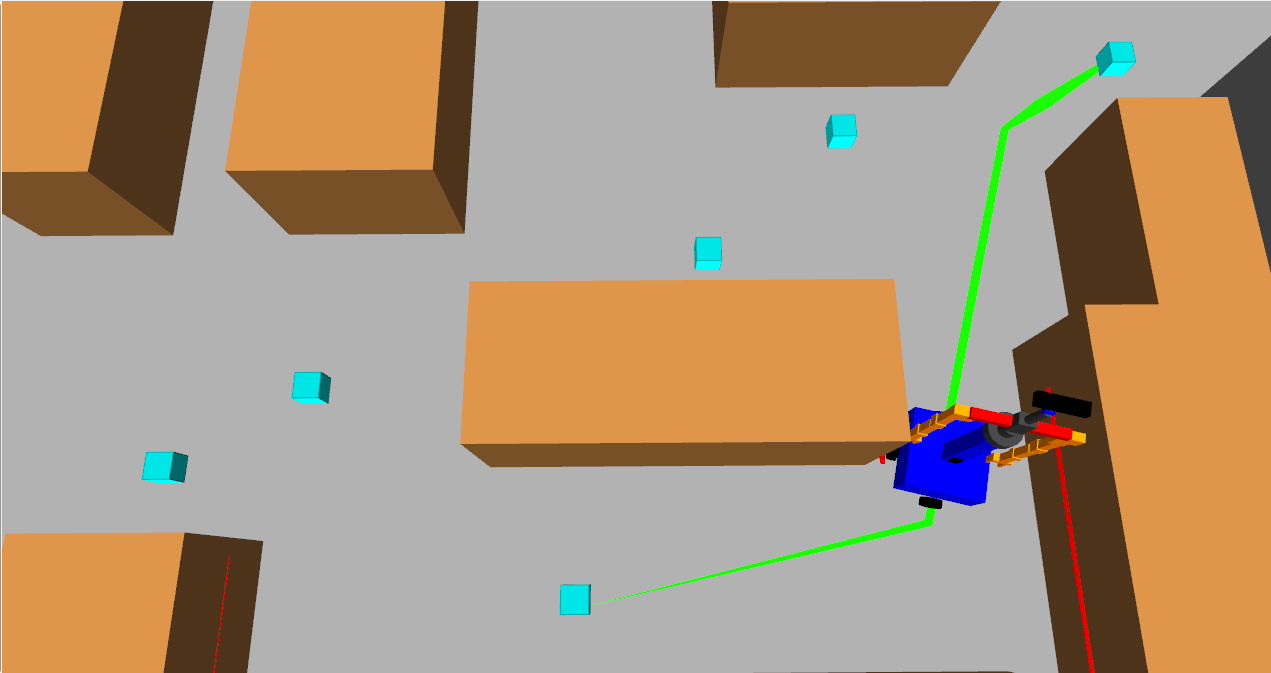
\includegraphics[width=\textwidth]{Figures/simulator1.png} 
		\caption{Path planning using an algorithm for a Topological Map.}
		\label{fig:Simulator1}
	\end{subfigure}
	\begin{subfigure}{0.49\textwidth}
		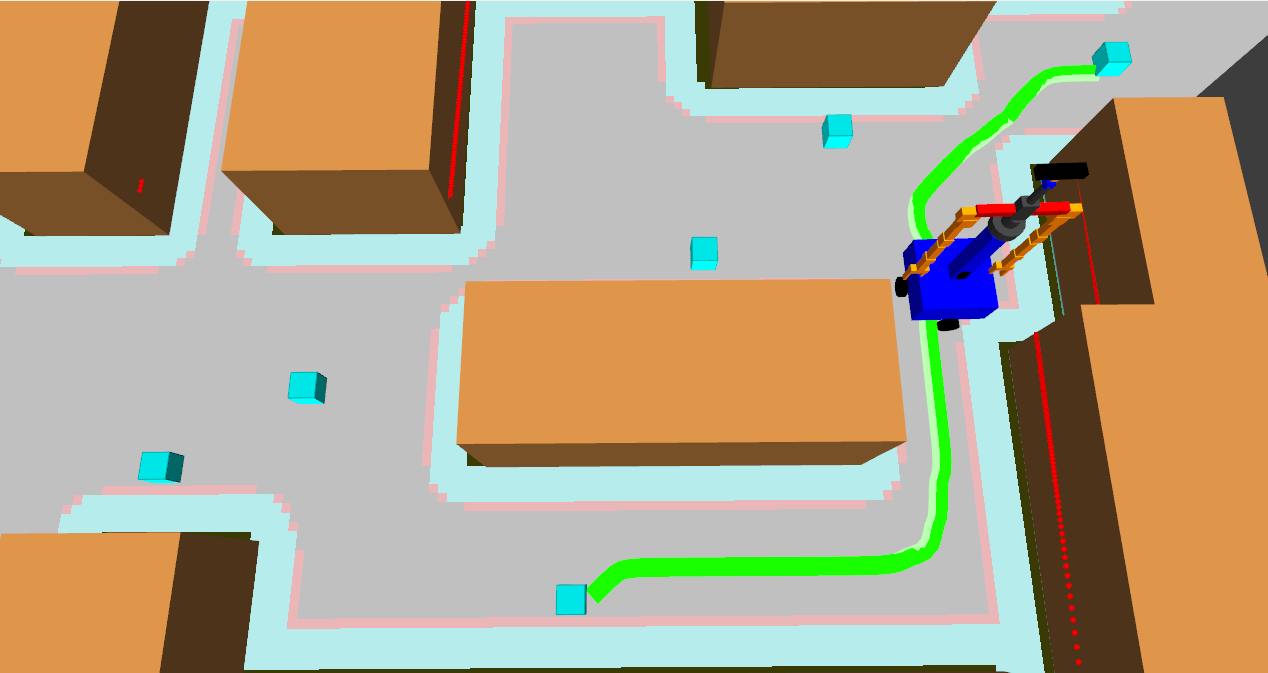
\includegraphics[width=\textwidth]{Figures/simulator2.png}
		\caption{Path planning using an algorithm for an Occupancy Grid.}
		\label{fig:Simulator2}
		\end{subfigure}
	\caption{Test of a navigation algorithm using the graphical interface of the simulator. }
	\label{fig:Simulator}
\end{figure}

Figure \ref{fig:Simulator1} shows the robot simulated, the virtual representation of our laboratory and a path created using Dijkstra Algorithm based on a topological representation of the environment. In contrast, Figure \ref{fig:Simulator2} shows a path created using the same robot and virtual environment, but using an Occupancy Grid instead for representing the map.

Thanks to the integration with ROS, after a simulation has been run, it allow us to test and visualize, in real time, the algorithms in robot Justina for result analysis and comparison. Different algorithms in a wide-range of environment configurations has been modelled and tested, both in simulation and in the real robot. 

%%% CHORO DEL SR. JULIO
\subsection{High level task planning using conceptual dependency}\label{subsec:ActionPln}
This year, a new knowledge based system for high level task planning has been developed. This system is designed for interpret a command in a natural language format and for generate a sequence of high level  actions that have to be completed to accomplish the command. With this system, the robot generates behaviours that can drive his own world representation, similarly to a human being. 

The system is composed by two principal modules:
\begin{description}
\item[Communication Module] In this module, the grammar structure of the commands is defined. Performs a syntactical analysis and a semantic interpretation using inferences and Conceptual Dependency, in order to find a meaning for the command. Finally, this module returns a formal expression that describe a sequence of high level actions that the robot have to execute. 
\item[Execution Module] Consist in a set of rules for infer and determinate the sequence of high level tasks as  basic and atomic predefined actions that represents the plan that will allow the robot to accomplish the command that has been requested. This module was developed using CLIPS, an expert system designed to represent and model the human knowledge.
\end{description}

\begin{figure}[H]
	\centering
	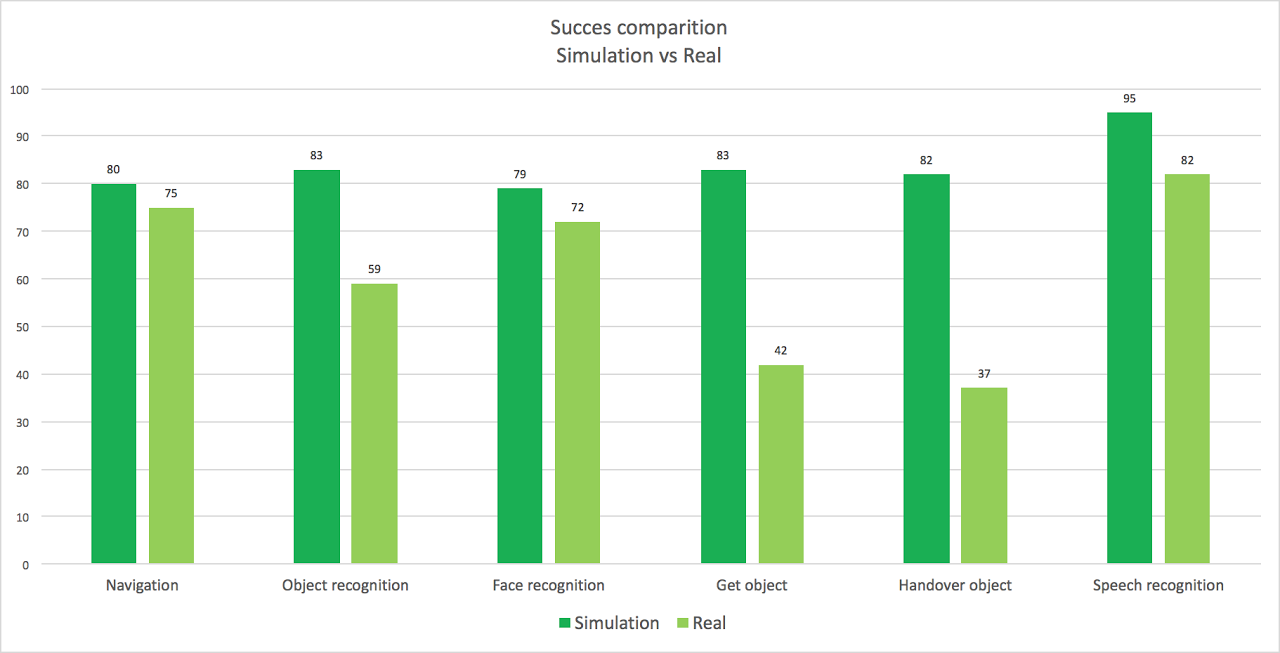
\includegraphics[width=0.8\textwidth]{Figures/taskPlanning.png}
	\caption{Comparison of success between simulated plans and real plans.}
	\label{fig:taskPlanning}
\end{figure}

We have compared the number of successfully executed plans, both in simulation and with the real robot, as can be seen in Figure \ref{fig:taskPlanning}, for 100 executions for each action.

So far, we have modelled actions like Navigation, Object Recognition, Face Recognition, Object Taking and Object Leaving.

%%% CHORO DEL SR. JESUS
\subsection{Low or null texture objects recognition using RGB-D cameras}\label{subsec:objDet}

Currently, several robust techniques based on feature extraction and description exist for object recognition. However, if the objects are low textured, only a few number of features can be extracted, making the matching process unreliable. For these cases, we developed a method that combine three characteristics: color, size and shape, combining the color and depth information for the recognition process, after a 3D detection and segmentation in a plane for each object.

Color Information is extracted from the HSV space of the object's pixels and it is represented by the histogram of the Hue component, but only for pixels with Saturation and Value above certain threshold. For pixels below these thresholds, two more bins are added to the histogram. For campaign histograms we used the histogram Intersection \cite{swain1991_HistoInter}.

The size and shape is estimated from the object's point cloud, which are obtained using an Oriented Bounding Box (OBB) of the point cloud as follow: the base of the OBB is obtained from the oriented bounding rectangle of the projection of the points in the plane below them. The heights are obtained from the maximum distance of the points to the plane. The shape is characterized using the Hu Moments \cite{hu1962_moments} of the convex hull calculated from the points projected over the plane below them. 

For the recognition process we compare in three steps: size, shape and color characteristics, removing candidates below a certain threshold for each step. At the end, from the remaining candidates, we select the best one according to a color-based similarity function. 

These method has been tested experimentally in the Rocking robotics competition, where the we obtained a second place in the ``object perception test'', showing fast and robust results for changes in light , scale, and rotation in a plane parallel to the plane below the object. Figure \ref{fig:objReco} shows an example of object recognition on a shelf (multiple planes).

\begin{figure}
	\centering
	\begin{subfigure}{0.49\textwidth}
		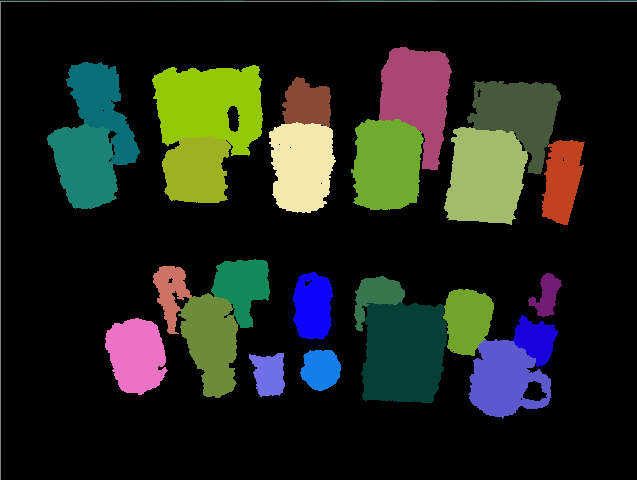
\includegraphics[width=\textwidth]{Figures/objetos2.png} 
		\caption{ Point clouds corresponding to each segmented object.}
		\label{fig:objReco1}
	\end{subfigure}
	\begin{subfigure}{0.49\textwidth}
		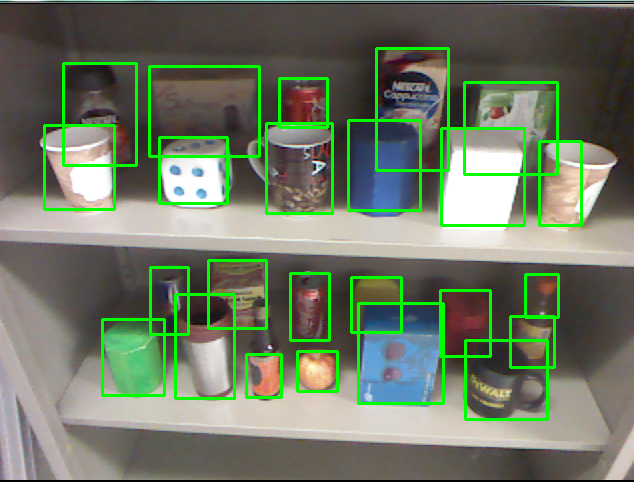
\includegraphics[width=\textwidth]{Figures/objetos1.png}
		\caption{Objects can be segmented even with occlusions.}
		\label{fig:objReco2}
	\end{subfigure}
	\caption{Example of object segmentation on several planes.}
	\label{fig:objReco}
\end{figure}



%%%%%%%%%%%%%%%%%%%%%%%%%%
%%%  CONCLUSION AND FUTURE WORK  %%%
%%%%%%%%%%%%%%%%%%%%%%%%%%

\section{Conclusions and future work}\label{sec:conclusions}

The ViRBot system and robot Justina has been successfully tested in RoboCup in the category @Home since the RoboCup competition of Atlanta 2007. The team has get into the finals the last two years (2014 and 2015) in this competition. Also, in 2014, the team participated in the RoCKIn Competition wining a 1st place and a $2^{nd}$ in different categories. In the 2015 edition of the same competition, the team won the second place in the ``Object perception'' test. Last year, in RoboCup 2017, the team got into the $2^{nd}$ stage.

In these years, the full system has been improved, both in hardware and software, having reliable performance and showing promising results. Particularly, this year, we have a new omnidirectional mobile base for navigation and a new torso. In terms of software, we have change the way of conceiving the tests of the competition: from state machines to inferences based on rules.  

As future work, we are trying to improve the computer vision algorithms to achieve real time detection and recognition of objects and persons. Also, we want to explore some methods for better path planning for object manipulation.


\bibliographystyle{unsrt}
\bibliography{References}
\end{document} 

%%% Local Variables:
%%% mode: latex
%%% TeX-master: t
%%% End:
